\documentclass[a4paper,12pt]{article}
\usepackage{graphicx}  
\usepackage{float}
\begin{document}
\pagenumbering{gobble}
\title{CEG2136 LAB 1 \\\ Group 21}
\author{Ryan Fleck - 8276723 \\\ Xiuzhu Li - 8571645}
\maketitle
\newpage
\pagenumbering{roman}
\tableofcontents
\listoffigures
\newpage
\pagenumbering{arabic}


\section{Theoretical Implementation}

\subsection{Lab Objectives}
The primary goal of this lab is to familiarize the student with the \textit{Altera DE2-115 FPGA} and it's companion software, \textit{Altera Quartus II}. The following objectives should be met:
\begin{enumerate}
\item Understand the basic of the Altera environment.
\item Design a simple logic circuit using the Graphic editor.
\item Compile, simulate, debug, and test their design.
\item Download and run their design on the Altera DE2-115 board.
\end{enumerate}

\subsection{Discussion of Requirements}
A circuit with the following logic function is to be implemented in \textit{Altera Quartus II} and run on the \textit{Altera DE2-115 FPGA}:
\begin{equation}
(A \cdot B)' + (C+D)'
\end{equation}

A derived truth table for this function can be found at the end of this document, \textbf{Figure \ref{fig:TruthTable1}}. The goal of the lab is to implement this circuit and have it run without errors on the \textit{Altera DE2-115 FPGA}, with every set of inputs resulting in the output predicted by the logic funciton and truth table.

\subsection{Proposed Algorithmic Solution}

As the equation \textbf{(1)} is already minimized, the equivalent logic gates will be used to construct the circuit. 
\begin{enumerate}
\item A NOR gate will be used to channel A and B.
\item A NAND gate will be used to channel C and D.
\item An AND gate will be used to process the output from the NAND and NOR gates.
\end{enumerate}

In total, three logical elements will be used. One each of NAND, NOR and AND gates. Please refer to \textit{Figure 2} in the \textit{CEG2136 Lab 1 Manual} for the original schematic the circuit is to be modeled after, and \textit{Altera Quartus II} part numbers. 




\section{Design}

\subsection{QUARTUS II Circuit Diagrams}

The circuit was implemented in \textit{Altera Quartus II} as shown in \textbf{Figure \ref{fig:Circ1}}.

\begin{figure}[H]
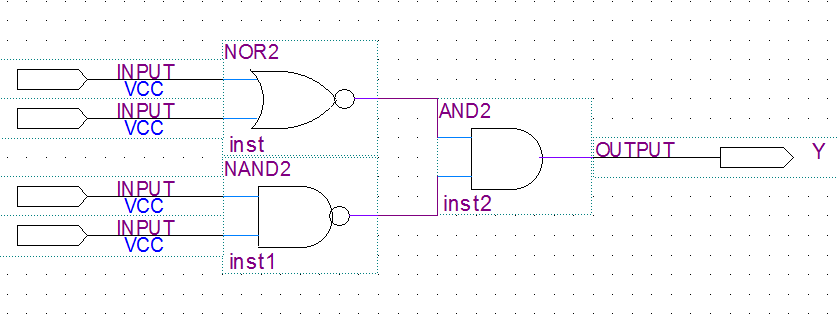
\includegraphics[width=\textwidth]{Images/Schematic2.PNG} 
\caption{Implemented Logical Circuit}
\label{fig:Circ1}
\end{figure}


\subsection{Components Utilized}

Our design, as shown in as shown in \textbf{Figure \ref{fig:Circ1}}, was implemented as intended with the components outlined in the \textit{Proposed Algorithmic Solution} subsection. No alternative components, that is, similar components with different part numbers (than those specified in the lab manual,) were used to create the logical circuit.

\subsection{Implemented Solution}
When implementing our solution, we took the following steps:
\begin{enumerate}
\item \textit{Altera Quartus II} was opened and the file was initialized.
\item The \textit{nor2, nand2} and \textit{and2} gates were selected and placed in the simulation without any problems, and joined together to adhere to the logical expression from the lab requirements \textbf{(1)}.
\item Pins were added and assigned correctly.
\item The file was compiled.
\item Pin numbers for the \textit{Altera DE2-115 'Cyclone' FPGA}, corresponding to logical inputs \textit{A, B, C, and D} were saved to the equivalent digital pins and LEDs within \textit{Altera Quartus II}.
\end{enumerate}
\subsection{Challenging Problems Encountered}

Some minor compilation errors occured at the beginning of the circuit's construction, but did not occur after the pin elements were placed on the digital schematic. We also had the classic error of being unable to see the \textit{USB Blaster} when initially trying to upload to the \textit{Altera DE2-115 FPGA} later in the experiment. No truly challenging problems were encountered when implementing \textbf{Figure \ref{fig:Circ1}}. It should be noted that the search function, though sometimes hidden in \textit{Altera Quartus II}, is very useful and came in handy during this lab. It is problematic that this program function was not used more often in ITI1100.





\section{Implementation}

\subsection{Simulation Results}
\textbf{Figure \ref{fig:Wav1}} shows a single set of 16 clock cycles, enough for PIN A to achieve a LOW voltage for 8 cycles, and a HIGH voltage for 8 more. As predicted by the KMAP derived in the prelab, and displayed in the appendices as \textbf{Figure \ref{fig:TruthTable1}}. This series of waveforms did not deviate from the waveform defined by our truth table and logical equations. 

\begin{figure}[H]
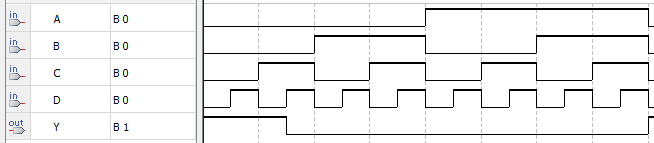
\includegraphics[width=\textwidth]{Images/Waveform2.PNG} 
\caption{Logical Circuit Waveform Output}
\label{fig:Wav1}
\end{figure}

\subsection{Simulation Verificaiton}
After recompiling, our \textit{Altera DE2-115 FPGA} had no issues simulating the circuit that had been designed. All 16 combinations of the 4 inputs were tested, and it was verified that the LED on the \textit{Altera DE2-115 FPGA} only responded with a HIGH voltage to the following combinations of the four inputs:

\begin{equation}
A'B'C'D'  ,  A'B'C'D  ,  A'B'CD'
\end{equation}


\section{Discussion}
After exhaustive testing of our running logical circuit, it was determined that it responded predictively to all possible input. There was no deviation from the behavior defined in \textbf{Figure \ref{fig:TruthTable1}} or our logic equations. There was no need to modify our circuit to fix deviant behaviour in the final waveform or physical implementation on the \textit{Altera DE2-115 FPGA}. It was fun to reminisce about ITI1100, and hopefully knowledge of the quirks in Altera's \textit{Quartus II} development environment will make the labs in this course smoother than those in that previous course.

\subsection{Errors Encountered}
\textbf{Figure \ref{fig:Uploaded}} shows our successful board upload. We had to reattempt the upload a few times, and had difficulty getting the lab computer to recognize the active \textit{Altera DE2-115 FPGA} connected via USB.
\begin{figure}[H]
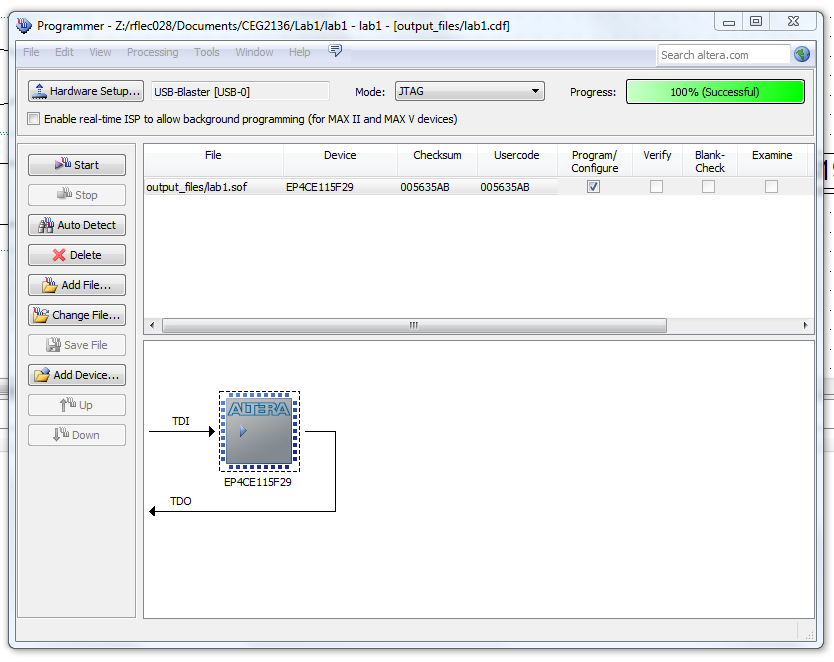
\includegraphics[width=\textwidth]{Images/Upload.PNG} 
\caption{Successful Upload to EP4CE115F29 Device.}
\label{fig:Uploaded}
\end{figure}


\subsection{Conclusions}
During lab 1 we recapped the course material of ITI1100, and once again found ourselves familiar with the \textit{Altera DE2-115 FPGA} along with its software, \textit{Quartus II}. Combinational circuits are a fundamental component of a robust computer engineering education. Mastering combinational circuits will allow more complex topics and digital circuits to be broken down more easily due to a depthful knowledge of the small-scale components. Lab 1 emphasizes the importance of logic gates' functionality, which are crucial to comprehending upcoming sequential circuits and more. Though straightforward, CEG2136 Lab 1 was a nice refresher and starting point to what we will encounter later in Computer Architecture I. We are looking forward to the challenge.

\newpage
\begin{figure}
\begin{center}
\caption{Truth Table for Logic Function 1}
\begin{tabular}{ |c|c|c|c||c| } 
 \hline
 A & B & C & D & Y\\
 \hline
 0 & 0 & 0 & 0 & 1\\
 0 & 0 & 0 & 1 & 1\\
 0 & 0 & 1 & 0 & 1\\
 0 & 0 & 1 & 1 & 0\\
 \hline
 0 & 1 & 0 & 0 & 0\\
 0 & 1 & 0 & 1 & 0\\
 0 & 1 & 1 & 0 & 0\\
 0 & 1 & 1 & 1 & 0\\
 \hline
 1 & 0 & 0 & 0 & 0\\
 1 & 0 & 0 & 1 & 0\\
 1 & 0 & 1 & 0 & 0\\
 1 & 0 & 1 & 1 & 0\\
 \hline
 1 & 1 & 0 & 0 & 0\\
 1 & 1 & 0 & 1 & 0\\
 1 & 1 & 1 & 0 & 0\\
 1 & 1 & 1 & 1 & 0\\
 \hline
\end{tabular}
\label{fig:TruthTable1}
\end{center}
\end{figure}

\newpage
\vspace*{\fill}
\center{\small Implemented by Ryan and Xiuzhu with \LaTeX.}

\end{document}





